\section{Модификация проекта <<Изображение проекции полиэдра>>}

\subsection{Постановка задачи}

Модифицируйте эталонный проект таким образом, чтобы определялась и печаталась следующая характеристика полиэдра: сумма длин рёбер, середина и ровно один из концов которых находится на расстоянии строго меньше $1$ от плоскости $x=2$. 
Для выполнения задания необходимо анализировать расположение середины и вершин всех ребер полиэдра относительно плоскости $x=2$. Для этого модифицируем эталонный проект, добавив необходимые методы нахождения середины ребра, расстояния от точки до плоскости $x=2$ и вычисления длины ребра.

\subsection{Решение задачи и модификация кода}
Чтобы определить, явялется ли точка хорошей, необходимо узнать находится ли координата $\mathit x$ любой точки на расстоянии строго меньше единицы от прямой $x=2$. Так как длина ~--- величина положительная будем использовать метод \texttt{abs}, позволяющий получить модуль числа, к которому применяется этот метод. Для определения, является ли точка удовлетворяющей условию, в классе \texttt{R3} файла \texttt{common/polyedr.rb}, добавим метод \texttt{good?}: 

\begin{small}
\begin{verbatim}
class R3
  ...
  def good?
    if (2.0 - @x).abs < 1.0 
      return true
    else
      return false
    end 
  end
  ...
\end{verbatim}
\end{small}

Ребро в нашем проекте является отрезком в пространстве, поэтому для нахождения середины ребра необходимо найти середину отрезка. Координаты середины отрезка в пространстве $[ \mathit a, \mathit b ]$ вычисляются по формуле:
$$x_{c}=\frac{a_{x}+b_{x}}{2};~y_{c}=~\frac{a_{y}+b_{y}}{2};~z_{c}=~ \frac{a_{z}+b_{z}}{2}.$$
В классе \texttt{Edge}, добавим метод, \texttt{center} который создает новую точку координаты которой находятся по формулам, указанным выше:

\begin{small}
\begin{verbatim}
class Edge
  ...
  def center
    xc=(@fin.x+@beg.x)/2.0 
    yc=(@fin.y+@beg.y)/2.0
    zc=(@fin.z+@beg.z)/2.0
    return R3.new(xc,yc,zc)
  end
  ...
\end{verbatim}
\end{small}


Так же добавим метод \texttt{length}, который возвращает длину ребра, где переменная \texttt{coef} явлется коэффициентом гомотетии.

\begin{small}
\begin{verbatim}
class Edge
  ...
  def length 
     Math.sqrt(((@fin.x-@beg.x)**2+(@fin.y-@beg.y)**2+(@fin.z-@beg.z)**2))/@coef
  end
  ...
\end{verbatim}
\end{small}

Далее добавим метод \texttt{func} в классе \texttt{Polyedr} возвращающий сумму длин рёбер, середина и ровно один из концов которых — «хорошие» точки.

\begin{small}
\begin{verbatim}
class Polyedr
  ...
  def func 
    sum=0
    edges.each do |e|
      if e.center.good?(e.coef) && (e.beg.good?(e.coef) ^ e.fin.good?(e.coef))
        sum += e.length
      end
    end
    return sum
  end
  ...
\end{verbatim}
\end{small}

После этого остается модифицировать файл, запускающий программу.

\begin{small}
\begin{verbatim}
#!/usr/bin/env ruby
# encoding: UTF-8
require './polyedr'
require '../common/tk_drawer'
TkDrawer.create
%w(test1 ).each do |name|
  puts '============================================================='
  puts "Начало работы с полиэдром '#{name}'"
  start_time = Time.now
  a=Polyedr.new("../data/#{name}.geom")
  a.draw 
  puts a.func
  puts "Изображение полиэдра '#{name}' заняло #{Time.now - start_time} сек."
  print 'Hit "Return" to continue -> '
  gets
end

\end{verbatim}
\end{small}

Модификация завершена. Работа программы с тестовым файлом \texttt{test1.geom} (рис.~6):

\begin{figure}[ht!]
\begin{center}
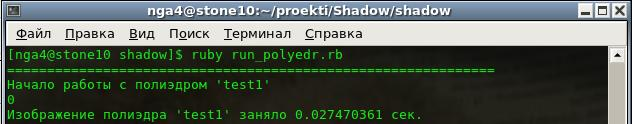
\includegraphics[scale=0.7]{images/6.jpg}
\center{\texttt{Рис.~6.}}
\end{center}
\end{figure}

Сам файл:

\begin{small}
\begin{verbatim}
10.0	0.0	0.0	0.0
4	1	4
1.5 0.0 0.0
3.5 0.0 0.0
3.5 5.0 0.0
1.5 5.0 0.0
4	1    2    3    4    
\end{verbatim}
\end{small}







